\chapter{Probability}

\index{probability}

A \key{probability} is a number between $0 \ldots 1$
that indicates how probable an event is.
If an event is certain to happen,
its probability is 1,
and if an event is impossible,
its probability is 0.

A typical example is throwing a dice,
where the result is an integer between
$1,2,\ldots,6$.
Usually it is assumed that the probability
for each result is $1/6$,
so all results have the same probability.

The probability of an event is denoted $P(\cdots)$
where the three dots are
a description of the event.
For example, when throwing a dice,
$P(\textrm{''the result is 4''})=1/6$,
$P(\textrm{''the result is not 6''})=5/6$
and $P(\textrm{''the result is even''})=1/2$.

\section{Calculation}

There are two standard ways to calculate
probabilities: combinatorial counting
and simulating a process.
As an example, let's calculate the probability
of drawing three cards with the same value
from a shuffled deck of cards
(for example, eight of spades,
eight of clubs and eight of diamonds).

\subsubsection*{Method 1}

We can calculate the probability using
the formula

\[\frac{\textrm{desired cases}}{\textrm{all cases}}.\]

In this problem, the desired cases are those
in which the value of each card is the same.
There are $13 {4 \choose 3}$ such cases,
because there are $13$ possibilities for the
value of the cards and ${4 \choose 3}$ ways to
choose $3$ suits from $4$ possible suits.

The number of all cases is ${52 \choose 3}$,
because we choose 3 cards from 52 cards.
Thus, the probability of the event is

\[\frac{13 {4 \choose 3}}{{52 \choose 3}} = \frac{1}{425}.\]

\subsubsection*{Method 2}

Another way to calculate the probability is
to simulate the process that generates the event.
In this case, we draw three cards, so the process
consists of three steps.
We require that each step in the process is successful.

Drawing the first card certainly succeeds,
because any card will do.
After this, the value of the cards has been fixed.
The second step succeeds with probability $3/51$,
because there are 51 cards left and 3 of them
have the same value as the first card.
Finally, the third step succeeds with probability $2/50$.

The probability that the entire process succeeds is

\[1 \cdot \frac{3}{51} \cdot \frac{2}{50} = \frac{1}{425}.\]

\section{Events}

An event in probability can be represented as a set
\[A \subset X,\]
where $X$ contains all possible outcomes,
and $A$ is a subset of outcomes.
For example, when drawing a dice, the outcomes are
\[X = \{x_1,x_2,x_3,x_4,x_5,x_6\},\]
where $x_k$ means the result $k$.
Now, for example, the event ''the result is even''
corresponds to the set
\[A = \{x_2,x_4,x_6\}.\]

Each outcome $x$ is assigned a probability $p(x)$.
Furthermore, the probability $P(A)$ of an event
that corresponds to a set $A$ can be calcuted as a sum
of probabilities of outcomes using the formula
\[P(A) = \sum_{x \in A} p(x).\]
For example, when throwing a dice,
$p(x)=1/6$ for each outcome $x$,
so the probability for the event
''the result is even'' is
\[p(x_2)+p(x_4)+p(x_6)=1/2.\]

The total probability of the outcomes in $X$ must
be 1, i.e., $P(X)=1$.

Since the events in probability are sets,
we can manipulate them using standard set operations:

\begin{itemize}
\item The \key{complement} $\bar A$ means
''$A$ doesn't happen''.
For example, when throwing a dice, 
the complement of $A=\{x_2,x_4,x_6\}$ is
$\bar A = \{x_1,x_3,x_5\}$.
\item The \key{union} $A \cup B$ means
''$A$ or $B$ happen''.
For example, the union of
$A=\{x_2,x_5\}$
and $B=\{x_4,x_5,x_6\}$ is
$A \cup B = \{x_2,x_4,x_5,x_6\}$.
\item The \key{intersection} $A \cap B$ means
''$A$ and $B$ happen''.
For example, the intersection of
$A=\{x_2,x_5\}$ and $B=\{x_4,x_5,x_6\}$ is
$A \cap B = \{x_5\}$.
\end{itemize}

\subsubsection{Complement}

The probability of the complement
$\bar A$ is calculated using the formula
\[P(\bar A)=1-P(A).\]

Sometimes, we can solve a problem easily
using complements by solving an opposite problem.
For example, the probability of getting
at least one six when throwing a dice ten times is
\[1-(5/6)^{10}.\]

Here $5/6$ is the probability that the result
of a single throw is not six, and
$(5/6)^{10}$ is the probability that none of
the ten throws is a six.
The complement of this is the answer for the problem.

\subsubsection{Union}

The probability of the union $A \cup B$
is calculated using the formula
\[P(A \cup B)=P(A)+P(B)-P(A \cap B).\]
For example, when throwing a dice,
the union of events
\[A=\textrm{''the result is even''}\]
and
\[B=\textrm{''the result is less than 4''}\]
is
\[A \cup B=\textrm{''the result is even or less than 4''},\]
and its probability is
\[P(A \cup B) = P(A)+P(B)-P(A \cap B)=1/2+1/2-1/6=5/6.\]

If the events $A$ and $B$ are \key{disjoint}, i.e.,
$A \cap B$ is empty,
the probability of the event $A \cup B$ is simply

\[P(A \cup B)=P(A)+P(B).\]

\subsubsection{Conditional probability}

\index{conditional probability}

The \key{conditional probability}
\[P(A | B) = \frac{P(A \cap B)}{P(B)}\]
is the probability of an event $A$
assuming that an event happens.
In this case, when calculating the
probability of $A$, we only consider the outcomes
that also belong to $B$.

Using the sets in the previous example,
\[P(A | B)= 1/3,\]
Because the outcomes in $B$ are
$\{x_1,x_2,x_3\}$, and one of them is even.
This is the probability of an even result
if we know that the result is between $1 \ldots 3$.

\subsubsection{Intersection}

\index{independence}

Using conditional probability,
the probability of the intersection
$A \cap B$ can be calculated using the formula
\[P(A \cap B)=P(A)P(B|A).\]
Events $A$ and $B$ are \key{independent} if
\[P(A|B)=P(A) \hspace{10px}\textrm{and}\hspace{10px} P(B|A)=P(B),\]
which means that the fact that $B$ happens doesn't
change the probability of $A$, and vice versa.
In this case, the probability of the intersection is
\[P(A \cap B)=P(A)P(B).\]
For example, when drawing a card from a deck, the events
\[A = \textrm{''the suit is clubs''}\]
and
\[B = \textrm{''the value is four''}\]
are independent. Hence the event
\[A \cap B = \textrm{''the card is the four of clubs''}\]
happens with probability
\[P(A \cap B)=P(A)P(B)=1/4 \cdot 1/13 = 1/52.\]

\section{Random variable}

\index{random variable}

A \key{random variable} is a value that is generated
by a random process.
For example, when throwing two dice,
a possible random variable is
\[X=\textrm{''the sum of the results''}.\]
For example, if the results are $(4,6)$,
then the value of $X$ is 10.

We denote $P(X=x)$ the probability that
the value of a random variable $X$ is $x$.
In the previous example, $P(X=10)=3/36$,
because the total number of results is 36,
and the possible ways to obtain the sum 10 are
$(4,6)$, $(5,5)$ and $(6,4)$.

\subsubsection{Expected value}

\index{expected value}

The \key{expected value} $E[X]$ indicates the
average value of a random variable $X$.
The expected value can be calculated as the sum
\[\sum_x P(X=x)x,\]
where $x$ goes through all possible results
for $X$.

For example, when throwing a dice,
the expected value is

\[1/6 \cdot 1 + 1/6 \cdot 2 + 1/6 \cdot 3 + 1/6 \cdot 4 + 1/6 \cdot 5 + 1/6 \cdot 6 = 7/2.\]

A useful property of expected values is \key{linearity}.
It means that the sum
$E[X_1+X_2+\cdots+X_n]$
always equals the sum
$E[X_1]+E[X_2]+\cdots+E[X_n]$.
This formula holds even if random variables
depend on each other.

For example, when throwing two dice,
the expected value of their sum is
\[E[X_1+X_2]=E[X_1]+E[X_2]=7/2+7/2=7.\]

Let's now consider a problem where
$n$ balls are randomly placed in $n$ boxes,
and our task is to calculate the expected
number of empty boxes.
Each ball has an equal probability to
be placed in any of the boxes.
For example, if $n=2$, the possibilities
are as follows:
\begin{center}
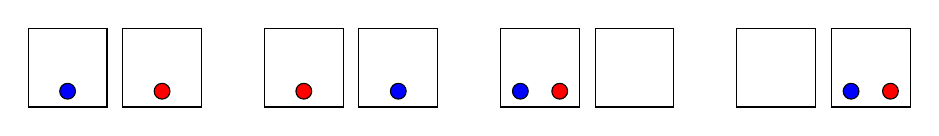
\begin{tikzpicture}
\draw (0,0) rectangle (1,1);
\draw (1.2,0) rectangle (2.2,1);
\draw (3,0) rectangle (4,1);
\draw (4.2,0) rectangle (5.2,1);
\draw (6,0) rectangle (7,1);
\draw (7.2,0) rectangle (8.2,1);
\draw (9,0) rectangle (10,1);
\draw (10.2,0) rectangle (11.2,1);

\draw[fill=blue] (0.5,0.2) circle (0.1);
\draw[fill=red] (1.7,0.2) circle (0.1);
\draw[fill=red] (3.5,0.2) circle (0.1);
\draw[fill=blue] (4.7,0.2) circle (0.1);
\draw[fill=blue] (6.25,0.2) circle (0.1);
\draw[fill=red] (6.75,0.2) circle (0.1);
\draw[fill=blue] (10.45,0.2) circle (0.1);
\draw[fill=red] (10.95,0.2) circle (0.1);
\end{tikzpicture}
\end{center}
In this case, the expected number of
empty boxes is
\[\frac{0+0+1+1}{4} = \frac{1}{2}.\]
In the general case, the probability that a
single box is empty is
\[\Big(\frac{n-1}{n}\Big)^n,\]
because no ball should be placed in it.
Hence, using linearity, the expected number of
empty boxes is
\[n \cdot \Big(\frac{n-1}{n}\Big)^n.\]

\subsubsection{Distributions}

\index{distribution}

The \key{distribution} of a random variable $X$
shows the probability for each value that
the random variable may have.
The distribution consists of values $P(X=x)$.
For example, when throwing two dice,
the distribution for their sum is:
\begin{center}
\small {
\begin{tabular}{r|rrrrrrrrrrrrr}
$x$ & 2 & 3 & 4 & 5 & 6 & 7 & 8 & 9 & 10 & 11 & 12 \\
$P(X=x)$ & $1/36$ & $2/36$ & $3/36$ & $4/36$ & $5/36$ & $6/36$ & $5/36$ & $4/36$ & $3/36$ & $2/36$ & $1/36$ \\
\end{tabular}
}
\end{center}

Next, we will discuss three distributions that
often arise in applications.

\index{uniform distribution}
~\\\\
In a \key{uniform distribution},
the value of a random variable is
between $a \ldots b$, and the probability
for each value is the same.
For example, throwing a dice generates
a uniform distribution where
$P(X=x)=1/6$ when $x=1,2,\ldots,6$.

The expected value for $X$ in a uniform distribution is
\[E[X] = \frac{a+b}{2}.\]
\index{binomial distribution}
~\\
In a \key{binomial distribution}, $n$ attempts
are done
and the probability that a single attempt succeeds
is $p$.
The random variable $X$ counts the number of
successful attempts,
and the probability for a value $x$ is
\[P(X=x)=p^x (1-p)^{n-x} {n \choose x},\]
where $p^x$ and $(1-p)^{n-x}$ correspond to
successful and unsuccessful attemps,
and ${n \choose x}$ is the number of ways
we can choose the order of the attempts.

For example, when throwing a dice ten times,
the probability of throwing a six exactly
three times is $(1/6)^3 (5/6)^7 {10 \choose 3}$.

The expected value for $X$ in a binomial distribution is
\[E[X] = pn.\]
\index{geometric distribution}
~\\
In a \key{geometric distribution},
the probability that an attempt succeeds is $p$,
and we do attempts until the first success happens.
The random variable $X$ counts the number
of attempts needed, and the probability for
a value $x$ is
\[P(X=x)=(1-p)^{x-1} p,\]
where $(1-p)^{x-1}$ corresponds to unsuccessful attemps
and $p$ corresponds to the first successful attempt.

For example, if we throw a dice until we throw a six,
the probability that the number of throws
is exactly 4 is $(5/6)^3 1/6$.

The expected value for $X$ in a geometric distribution is
\[E[X]=\frac{1}{p}.\]

\section{Markovin ketju}

\index{Markovin ketju@Markovin ketju}

\key{Markovin ketju} on satunnaisprosessi,
joka muodostuu tiloista ja niiden välisistä siirtymistä.
Jokaisesta tilasta tiedetään, millä todennäköisyydellä
siitä siirrytään toisiin tiloihin.
Markovin ketju voidaan esittää verkkona,
jonka solmut ovat tiloja
ja kaaret niiden välisiä siirtymiä.

Tarkastellaan esimerkkinä tehtävää,
jossa olet alussa $n$-kerroksisen
rakennuksen kerroksessa 1.
Joka askeleella liikut satunnaisesti
kerroksen ylöspäin tai alaspäin,
paitsi kerroksesta 1 liikut aina ylöspäin
ja kerroksesta $n$ aina alaspäin.
Mikä on todennäköisyys, että olet $m$
askeleen jälkeen kerroksessa $k$?

Tehtävässä kukin rakennuksen kerros
on yksi tiloista, ja kerrosten välillä liikutaan
satunnaisesti.
Esimerkiksi jos $n=5$, verkosta tulee:

\begin{center}
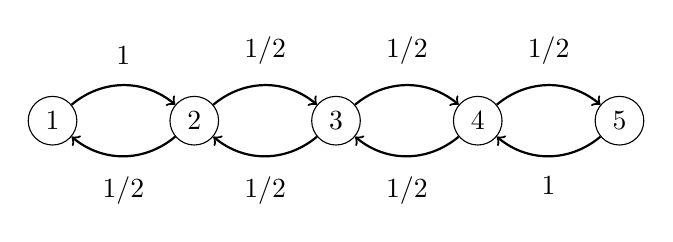
\begin{tikzpicture}[scale=0.9]
\node[draw, circle] (1) at (0,0) {$1$};
\node[draw, circle] (2) at (2,0) {$2$};
\node[draw, circle] (3) at (4,0) {$3$};
\node[draw, circle] (4) at (6,0) {$4$};
\node[draw, circle] (5) at (8,0) {$5$};

\path[draw,thick,->] (1) edge [bend left=40] node[font=\small,label=$1$] {} (2);
\path[draw,thick,->] (2) edge [bend left=40] node[font=\small,label=$1/2$] {} (3);
\path[draw,thick,->] (3) edge [bend left=40] node[font=\small,label=$1/2$] {} (4);
\path[draw,thick,->] (4) edge [bend left=40] node[font=\small,label=$1/2$] {} (5);

\path[draw,thick,->] (5) edge [bend left=40] node[font=\small,label=below:$1$] {} (4);
\path[draw,thick,->] (4) edge [bend left=40] node[font=\small,label=below:$1/2$] {} (3);
\path[draw,thick,->] (3) edge [bend left=40] node[font=\small,label=below:$1/2$] {} (2);
\path[draw,thick,->] (2) edge [bend left=40] node[font=\small,label=below:$1/2$] {} (1);

%\path[draw,thick,->] (1) edge [bend left=40] node[font=\small,label=below:$1$] {} (2);
\end{tikzpicture}
\end{center}

Markovin ketjun tilajakauma on vektori
$[p_1,p_2,\ldots,p_n]$, missä $p_k$ tarkoittaa
todennäköisyyttä olla tällä hetkellä tilassa $k$.
Todennäköisyyksille pätee aina $p_1+p_2+\cdots+p_n=1$.

Esimerkissä jakauma on ensin $[1,0,0,0,0]$,
koska on varmaa, että kulku alkaa kerroksesta 1.
Seuraava jakauma on $[0,1,0,0,0]$,
koska kerroksesta 1 pääsee vain kerrokseen 2.
Tämän jälkeen on mahdollisuus mennä joko ylöspäin
tai alaspäin, joten seuraava jakauma on $[1/2,0,1/2,0,0]$, jne.

Tehokas tapa simuloida kulkua Markovin ketjussa
on käyttää dynaamista ohjelmointia.
Ideana on pitää yllä tilajakaumaa
ja käydä joka vuorolla läpi kaikki tilat
ja jokaisesta tilasta kaikki mahdollisuudet jatkaa eteenpäin.
Tätä menetelmää käyttäen $m$ askeleen simulointi
vie aikaa $O(n^2 m)$.

Markovin ketjun tilasiirtymät voi esittää myös matriisina,
jonka avulla voi päivittää tilajakaumaa askeleen eteenpäin.
Tässä tapauksessa matriisi on

\[ 
 \begin{bmatrix}
  0 & 1/2 & 0 & 0 & 0 \\
  1 & 0 & 1/2 & 0 & 0 \\
  0 & 1/2 & 0 & 1/2 & 0 \\
  0 & 0 & 1/2 & 0 & 1 \\
  0 & 0 & 0 & 1/2 & 0 \\
 \end{bmatrix}.
\]

Tällaisella matriisilla voi kertoa tilajakaumaa esittävän
vektorin, jolloin saadaan tilajakauma yhtä askelta myöhemmin.
Esimerkiksi jakaumasta $[1,0,0,0,0]$ pääsee jakaumaan
$[0,1,0,0,0]$ seuraavasti:

\[ 
 \begin{bmatrix}
  0 & 1/2 & 0 & 0 & 0 \\
  1 & 0 & 1/2 & 0 & 0 \\
  0 & 1/2 & 0 & 1/2 & 0 \\
  0 & 0 & 1/2 & 0 & 1 \\
  0 & 0 & 0 & 1/2 & 0 \\
 \end{bmatrix}
 \begin{bmatrix}
  1 \\
  0 \\
  0 \\
  0 \\
  0 \\
 \end{bmatrix}
=
 \begin{bmatrix}
  0 \\
  1 \\
  0 \\
  0 \\
  0 \\
 \end{bmatrix}.
\]

Matriisiin voi soveltaa edelleen tehokasta
matriisipotenssia, jonka avulla voi laskea
ajassa $O(n^3 \log m)$,
mikä on jakauma $m$ askeleen jälkeen.

\section{Satunnaisalgoritmit}

\index{satunnaisalgoritmi@satunnaisalgoritmi}

Joskus tehtävässä voi hyödyntää satunnaisuutta,
vaikka tehtävä ei itsessään liittyisi todennäköisyyteen.
\key{Satunnaisalgoritmi} on algoritmi, jonka toiminta
perustuu satunnaisuuteen.

\index{Monte Carlo -algoritmi}

\key{Monte Carlo -algoritmi} on satunnaisalgoritmi,
joka saattaa tuottaa joskus väärän tuloksen.
Jotta algoritmi olisi käyttökelpoinen,
väärän vastauksen todennäköisyyden tulee olla pieni.

\index{Las Vegas -algoritmi}

\key{Las Vegas -algoritmi} on satunnaisalgoritmi,
joka tuottaa aina oikean tuloksen mutta jonka
suoritusaika vaihtelee satunnaisesti.
Tavoitteena on, että algoritmi toimisi nopeasti
suurella todennäköisyydellä.

Tutustumme seuraavaksi kolmeen esimerkkitehtävään,
jotka voi ratkaista satunnaisuuden avulla.

\subsubsection{Järjestystunnusluku}

\index{järjestystunnusluku}

Taulukon $k$. \key{järjestystunnusluku}
on kohdassa $k$ oleva alkio,
kun alkiot järjestetään
pienimmästä suurimpaan.
On helppoa laskea mikä tahansa
järjestystunnusluku ajassa $O(n \log n)$
järjestämällä taulukko,
mutta onko oikeastaan tarpeen järjestää koko taulukkoa?

Osoittautuu, että järjestystunnusluvun
voi etsiä satunnaisalgoritmilla ilman taulukon
järjestämistä.
Algoritmi on Las Vegas -tyyppinen:
sen aikavaativuus on yleensä $O(n)$,
mutta pahimmassa tapauksessa $O(n^2)$.

Algoritmi valitsee taulukosta satunnaisen alkion $x$
ja siirtää $x$:ää pienemmät alkiot
taulukon vasempaan osaan ja loput alkiot
taulukon oikeaan osaan.
Tämä vie aikaa $O(n)$, kun taulukossa on $n$ alkiota.
Oletetaan, että vasemmassa osassa on $a$
alkiota ja oikeassa osassa on $b$ alkiota.
Nyt jos $a=k-1$, alkio $x$ on haluttu alkio.
Jos $a>k-1$, etsitään rekursiivisesti
vasemmasta osasta, mikä on kohdassa $k$ oleva alkio.
Jos taas $a<k-1$, etsitään rekursiivisesti
oikeasta osasta, mikä on kohdassa $k-a-1$ oleva alkio.
Haku jatkuu vastaavalla tavalla rekursiivisesti,
kunnes haluttu alkio on löytynyt.

Kun alkiot $x$ valitaan satunnaisesti,
taulukon koko suunnilleen puolittuu
joka vaiheessa, joten kohdassa $k$ olevan
alkion etsiminen vie aikaa
\[n+n/2+n/4+n/8+\cdots=O(n).\]

Algoritmin pahin tapaus on silti $O(n^2)$,
koska on mahdollista,
että $x$ valitaan sattumalta aina niin,
että se on taulukon pienin alkio.
Silloin taulukko pienenee joka vaiheessa
vain yhden alkion verran.
Tämän todennäköisyys on kuitenkin erittäin pieni,
eikä näin tapahdu käytännössä.

\subsubsection{Matriisitulon tarkastaminen}

\index{matriisitulo@matriisitulo}

Seuraava tehtävämme on \emph{tarkastaa},
päteekö matriisitulo $AB=C$, kun $A$, $B$ ja $C$
ovat $n \times n$ -kokoisia matriiseja.
Tehtävän voi ratkaista laskemalla matriisitulon
$AB$ (perusalgoritmilla ajassa $O(n^3)$), mutta voisi toivoa,
että ratkaisun tarkastaminen olisi helpompaa
kuin sen laskeminen alusta alkaen uudestaan.

Osoittautuu, että tehtävän voi ratkaista
Monte Carlo -algoritmilla,
jonka aikavaativuus on vain $O(n^2)$.
Idea on yksinkertainen: valitaan satunnainen
$n \times 1$ -matriisi $X$ ja lasketaan
matriisit $ABX$ ja $CX$.
Jos $ABX=CX$, ilmoitetaan, että $AB=C$,
ja muuten ilmoitetaan, että $AB \neq C$.

Algoritmin aikavaativuus on $O(n^2)$,
koska matriisien $ABX$ ja $CX$ laskeminen
vie aikaa $O(n^2)$.
Matriisin $ABX$ tapauksessa laskennan
voi suorittaa osissa $A(BX)$, jolloin riittää
kertoa kahdesti $n \times n$- ja $n \times 1$-kokoiset
matriisit.

Algoritmin heikkoutena on, että on pieni mahdollisuus,
että algoritmi erehtyy, kun se ilmoittaa, että $AB=C$.
Esimerkiksi 
\[
 \begin{bmatrix}
  2 & 4 \\
  1 & 6 \\
 \end{bmatrix}
\neq
 \begin{bmatrix}
  0 & 5 \\
  7 & 4 \\
 \end{bmatrix},
\]
mutta
\[
 \begin{bmatrix}
  2 & 4 \\
  1 & 6 \\
 \end{bmatrix}
 \begin{bmatrix}
  1 \\
  3 \\
 \end{bmatrix}
=
 \begin{bmatrix}
  0 & 5 \\
  7 & 4 \\
 \end{bmatrix}
 \begin{bmatrix}
  1 \\
  3 \\
 \end{bmatrix}.
\]
Käytännössä erehtymisen todennäköisyys on kuitenkin
pieni ja todennäköisyyttä voi pienentää lisää
tekemällä tarkastuksen usealla
satunnaisella matriisilla $X$ ennen vastauksen
$AB=C$ ilmoittamista.

\subsubsection{Verkon värittäminen}

\index{vxritys@väritys}

Annettuna on verkko, jossa on $n$ solmua ja $m$ kaarta.
Tehtävänä on etsiä tapa värittää verkon solmut kahdella värillä
niin, että ainakin $m/2$ kaaressa
päätesolmut ovat eri väriset.
Esimerkiksi verkossa
\begin{center}
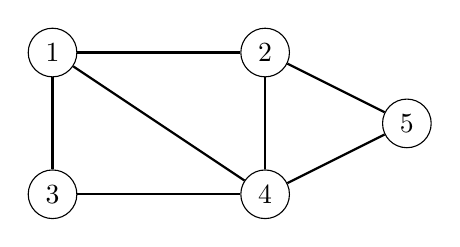
\begin{tikzpicture}[scale=0.9]
\node[draw, circle] (1) at (1,3) {$1$};
\node[draw, circle] (2) at (4,3) {$2$};
\node[draw, circle] (3) at (1,1) {$3$};
\node[draw, circle] (4) at (4,1) {$4$};
\node[draw, circle] (5) at (6,2) {$5$};

\path[draw,thick,-] (1) -- (2);
\path[draw,thick,-] (1) -- (3);
\path[draw,thick,-] (1) -- (4);
\path[draw,thick,-] (3) -- (4);
\path[draw,thick,-] (2) -- (4);
\path[draw,thick,-] (2) -- (5);
\path[draw,thick,-] (4) -- (5);
\end{tikzpicture}
\end{center}
yksi kelvollinen väritys on seuraava:
\begin{center}
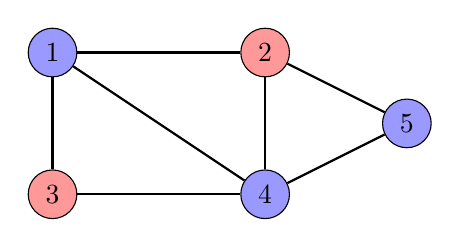
\begin{tikzpicture}[scale=0.9]
\node[draw, circle, fill=blue!40] (1) at (1,3) {$1$};
\node[draw, circle, fill=red!40] (2) at (4,3) {$2$};
\node[draw, circle, fill=red!40] (3) at (1,1) {$3$};
\node[draw, circle, fill=blue!40] (4) at (4,1) {$4$};
\node[draw, circle, fill=blue!40] (5) at (6,2) {$5$};

\path[draw,thick,-] (1) -- (2);
\path[draw,thick,-] (1) -- (3);
\path[draw,thick,-] (1) -- (4);
\path[draw,thick,-] (3) -- (4);
\path[draw,thick,-] (2) -- (4);
\path[draw,thick,-] (2) -- (5);
\path[draw,thick,-] (4) -- (5);
\end{tikzpicture}
\end{center}
Yllä olevassa verkossa on 7 kaarta ja niistä 5:ssä
päätesolmut ovat eri väriset,
joten väritys on kelvollinen.

Tehtävä on mahdollista ratkaista Las Vegas -algoritmilla
muodostamalla satunnaisia värityksiä niin kauan,
kunnes syntyy kelvollinen väritys.
Satunnaisessa värityksessä jokaisen solmun väri on
valittu toisistaan riippumatta niin,
että kummankin värin todennäköisyys on $1/2$.

Satunnaisessa värityksessä todennäköisyys, että yksittäisen kaaren päätesolmut
ovat eri väriset on $1/2$. Niinpä odotusarvo, monessako kaaressa
päätesolmut ovat eri väriset, on $1/2 \cdot m = m/2$.
Koska satunnainen väritys on odotusarvoisesti kelvollinen,
jokin kelvollinen väritys löytyy käytännössä nopeasti.

